\documentclass[conference]{IEEEtran}
\IEEEoverridecommandlockouts
\usepackage{cite}
\usepackage{amsmath,amssymb,amsfonts}
\usepackage{algorithmic}
\usepackage{graphicx}
\usepackage{textcomp}
\usepackage{xcolor}
\usepackage{booktabs}
\usepackage{siunitx}
\sisetup{detect-all}
\setlength{\textfloatsep}{4pt plus 2pt minus 2pt}
\setlength{\floatsep}{3pt plus 2pt minus 2pt}
\setlength{\intextsep}{5pt plus 2pt minus 2pt}
\setlength{\abovecaptionskip}{2pt}
\setlength{\belowcaptionskip}{0pt}
\renewcommand{\arraystretch}{0.88}
\linespread{0.955}\selectfont
\usepackage{titlesec}
\titlespacing*{\section}{0pt}{1.6ex plus .3ex minus .2ex}{0.9ex}
\titlespacing*{\subsection}{0pt}{1.1ex plus .2ex minus .2ex}{0.6ex}
\def\BibTeX{{\rm B\kern-.05em{\sc i\kern-.025em b}\kern-.08em
    T\kern-.1667em\lower.7ex\hbox{E}\kern-.125emX}}
\begin{document}
\title{Hardware-Oriented Compression of a Neural Decoder for Bivariate
Bicycle Codes:\\
Low-Bit Quantization and Activation Sparsity}
\author{\IEEEauthorblockN{Alan Daleth Hernandez Barreto}
\IEEEauthorblockA{\textit{Tecnol\'ogico Nacional de M\'exico}\\
\textit{Instituto Tecnol\'ogico de Zacatepec}\\
Zacatepec, Morelos, Mexico \\
\texttt{L23090959@zacatepec.tecnm.mx}}
}
\maketitle
\begin{abstract}
Real-time decoding is one of the dominant obstacles to fault-tolerant
quantum computing: the decoder must process syndrome data within the
microsecond-scale feedback latency of the quantum processor, under tight
area and power budgets. Neural decoders based on attention achieve the
best known accuracy for bivariate bicycle (BB) codes, but their
floating-point cost is far above what an on-chip accelerator can afford.
In this work we characterize, in a post-training setting, how
aggressively a state-of-the-art pretrained transformer decoder for a
$[[72,12,6]]$ BB code can be compressed without losing correction
accuracy. Using symmetric per-output-channel weight quantization and
per-token activation quantization, we observe that 8-bit weights and
activations (W8A8) preserve accuracy within the $95\%$ sampling
uncertainty, and that 4-bit weights with 8-bit activations (W4A8) degrade
accuracy only marginally, whereas 4-bit activations collapse accuracy. We
further show that a magnitude threshold can gate off roughly $28$--$37\%$
of activation values with no measurable accuracy loss. We also report a
negative experimental result: a naive post-training replacement of the
smooth activations (GELU/SiLU) by a rectifier, a first step towards
spiking and event-driven hardware, severely degrades decoding. We then
show that a short quantization-aware training pass recovers these
collapsed configurations by more than an order of magnitude, indicating
that the post-training constraint is a training rather than an intrinsic
limit. Together with analytical hardware cost estimates, these results
delineate the post-training operating point for low-power neural QEC
decoders and motivate quantization-aware training for truly event-driven
operation.
\end{abstract}
\begin{IEEEkeywords}
quantum error correction, bivariate bicycle codes, neural decoder,
low-bit quantization, activation sparsity, hardware-oriented machine
learning
\end{IEEEkeywords}
\section{Introduction}
Quantum error correction (QEC) requires a classical decoder that consumes
the syndrome measurements produced every cycle by the quantum processor and
returns a correction before the next cycle. For surface-code experiments
the decoding budget is on the order of one microsecond per round, and
meeting this target while remaining accurate is a central engineering
problem for real-time QEC \cite{dennis2002,google2023}.
Bivariate bicycle (BB) codes \cite{bravyi2024} are a family of quantum
low-density parity-check (QLDPC) codes with high encoding rate and short
check weight, and they are strong candidates for low-overhead fault
tolerance. Their decoding is difficult for belief propagation, and neural
decoders have been shown to outperform classical baselines on these codes
\cite{blue2026,LiuDiff25,CaoGen25,MiMueller25}. Among the most accurate reported decoders are attention-based
transformers that operate directly on the full syndrome history.
The main drawback of neural decoders is their cost: the reference decoder
here has ~36M parameters and performs many floating-point matrix
multiplications per syndrome, incompatible with the area and power
envelope of a cryogenic or edge accelerator. Two hardware-oriented techniques can mitigate this cost:
(i)~numerical precision, i.e.\ few-bit weights and activations, and
(ii)~activation sparsity, i.e.\ skipping operations with zero inputs---both
prerequisites for the event-driven accelerators that promise low-power
inference.
In this paper we characterize how far these two levers can be pushed on a
pretrained transformer decoder for a $[[72,12,6]]$ BB code without
retraining, i.e.\ in a post-training setting, and then ask whether a
short quantization-aware training pass can close the residual gap. Our
contributions are:
\begin{itemize}
\item a post-training bit-width sweep (down to ternary weights and 4-bit
      activations) on a faithful BB task, with $95\%$ Wilson intervals;
\item a measurement of accuracy-preserving activation sparsity from a
      simple magnitude threshold;
\item analytical estimates of the memory, arithmetic-energy, and
      operation-count reductions relative to FP32;
\item a negative result: a naive GELU/SiLU\,$\rightarrow$\,ReLU
      replacement, a first step towards spiking hardware, degrades
      accuracy;
\item a demonstration that a short quantization-aware training (QAT)
      pass recovers the collapsed rectifier/LIF configurations by more
      than an order of magnitude, confirming the constraint is a training
      rather than an intrinsic problem.
\end{itemize}
To the best of our knowledge, we are not aware of any prior systematic study of post-training compression limits for attention-based BB/QLDPC neural decoders;
existing compression results for neural QEC decoders target surface codes
and rely on quantization-aware training. All experiments use 5000 sampled
syndromes per noise level on a faithful circuit (except the
quantization-aware training study, which uses an independent 3000-shot
validation set), with the standard
block-level logical error rate (LER) over $K{=}12$ logical qubits as the
metric.
\section{Background}\label{sec:bg}
\subsection{Bivariate Bicycle Codes}
A BB code is defined by two commuting circulant matrices over
$\mathbb{Z}$, giving a CSS quantum stabilizer code with a Tanner graph of
bounded degree. We consider the $[[72,12,6]]$ code targeted by the
pretrained checkpoint used in this study, which encodes $K{=}12$ logical
qubits with a 432-bit detector set per sample over 6 syndrome-extraction
rounds under a circuit-level depolarizing noise model generated with
\texttt{stim} \cite{stimb}. The noise parameter $p$ is the physical error
rate per operation; the metric is the block logical error rate, the
probability that at least one of the 12 logical bits is decoded
incorrectly.
\subsection{Reference Neural Decoder}
Alongside recent generative, diffusion, and generalizable QLDPC neural
decoders~\cite{LiuDiff25,CaoGen25,MiMueller25}, our starting point is the
pretrained attention-based transformer decoder of Blue \emph{et al.}~\cite{blue2026},
released as an open checkpoint. The network interleaves recurrent spatial
blocks with cross-attention over the syndrome history and uses gated
(SwiGLU-style) feed-forward layers with smooth GELU/SiLU activations; it
outputs $K{=}12$ logits whose sign gives the correction. It has 35.98M
parameters and was trained to 10500 steps, and we treat it as a fixed
reference.
\subsection{Hardware Constraints}
Real-time decoding has strict latency and area budgets~\cite{DasHPCA22},
motivating the techniques explored here---few-bit integer arithmetic and
activation sparsity---exactly those exploited by integer and event-driven
accelerators, making them a natural first step towards deployable QEC
decoders. Prior work found that aggressive activation precision requires
quantization-aware training to remain accurate \cite{rethink2026}; we
measure the post-training boundary of this trade-off for the BB
transformer.
\section{Methodology}\label{sec:method}
We apply inference-time (post-training) transformations to the frozen
network, simulated in floating point with round-to-nearest assignment, so
the numbers reflect the behavior integer hardware would exhibit,
excluding accumulator effects, which we do not model.

\subsection{Weight Quantization}
For each weight tensor we use symmetric uniform quantization per output
channel: with $q=2^{b-1}-1$ and scale $s_o=\max|\mathbf{W}_o|/q$, the
quantized weight is\begin{equation}
\hat{\mathbf{W}}_o = s_o \cdot
\operatorname{round}\!\left(\mathbf{W}_o / s_o\right),
\end{equation}clipped to $[-q,q]$, where $\mathbf{W}_o$ collects the weights of output
channel $o$. Ternary weights use $\{-1,0,+1\}$ with a per-channel scale,
the extreme low-precision case. This needs one scale per output channel
and no zero-point, the cheapest configuration for hardware.
\subsection{Activation Quantization}
Activations are quantized per token (per row of the activation matrix)
with a symmetric scale set by the maximum absolute value in that row; this
dynamic scheme adapts to the varying activation magnitudes across tokens
while remaining streaming-friendly. Biases and normalization parameters
are kept in higher precision.
\subsection{Activation Sparsity}
To emulate event-driven execution we gate activations by magnitude: an
activation $a$ is forwarded only if $|a|>\tau$, otherwise it is set to
zero. We report the resulting \emph{activation fraction}, i.e.\ the
fraction of post-activation values that remain non-zero, which upper-bounds
the fraction of multiply-accumulate (MAC) operations that an event-driven
engine would execute. A range of magnitude thresholds $\tau$ is swept to
locate where sparsity begins to cost accuracy.
\subsection{Activation-Function Replacement}
Spiking and most event-driven neuron models use a rectifier-like transfer
function rather than the smooth GELU/SiLU used by the transformer. To
estimate how far the pretrained model is from such hardware, we replace
every GELU/SiLU by a rectifier at inference time and re-measure accuracy,
both in full precision and combined with W8A8 and W4A8 quantization.
Following the standard surrogate-gradient formulation for
spiking neurons, we model the target behavior with the continuous
soft-threshold surrogate gate
$$\begin{equation}
s(x)=x\,\sigma(x-\theta), \qquad \sigma(z)=\frac{1}{1+e^{-z}}.
\end{equation}
instead of implementing a discrete Leaky Integrate-and-Fire (LIF) unit in
the forward pass. This gate remains differentiable while approximating a
rectifying transfer function for $\theta>0$. At $\theta=0$,
$s(x)=x\sigma(x)=\text{SiLU}(x)$, which differs from the original
$\text{GELU}(x)=x\Phi(x)$ in both functional form and slope
($\Phi$ is the standard normal CDF). Because the pretrained checkpoint was
calibrated with GELU, substituting GELU by $\text{SiLU}(x)$
post-training shifts the activation distribution and accounts for the
large accuracy drop observed in Table~\ref{tab:qat}. We therefore treat
$s(x)$ as a \emph{continuous surrogate} for a rectifying neuron, not a
claim of equivalence to the smooth activations; true discrete spiking is
deferred to the quantization-aware training setting, where the network can
re-calibrate to this nonlinearity.
\section{Results}\label{sec:results}
All evaluations use 5000 sampled syndromes per noise level on the faithful
BB circuit, except the quantization-aware training study, which uses an
independent 3000-shot validation set; we report Wilson $95\%$ confidence
intervals (CI). Because
the CI on a low-$p$ logical error rate is wide, claims of ``no
degradation'' are supported by a two-proportion $z$-test as well.
\subsection{Reference Accuracy}
Table~\ref{tab:ref} reports the accuracy of the unmodified transformer
decoder together with the BP-OSD baseline. At $p{=}0.003$ the transformer
achieves a block LER of $5.8\times10^{-3}$ versus $7.87\times10^{-2}$ for
correlated BP-OSD on the same task, consistent with the order-of-magnitude
improvement reported for this family of codes \cite{blue2026}. This
confirms that the checkpoint reproduces state-of-the-art BB decoding and is
a meaningful platform for a compression study. The FP32 entry of
Table~\ref{tab:quant} is an independent 5000-shot resampling of the same
frozen model (26 vs 29 of 5000 shots), well within sampling noise.
\begin{table}[t]
\caption{Reference accuracy of the pretrained transformer decoder on the
faithful $[[72,12,6]]$ circuit (5000 shots per noise level, block LER over
$K{=}12$ logicals). Correlated BP-OSD at
$p{=}0.003$ is $7.87\times10^{-2}$. Wilson $95\%$ CIs of the compressed
configurations are given in Tables~\ref{tab:quant} and~\ref{tab:sparse}.}
\label{tab:ref}
\centering
\begin{tabular}{ccc}
\toprule
$p$ & Transformer LER & BP-OSD uncorr. \\
\midrule
0.001 & $2.0\times10^{-4}$ & $2.0\times10^{-4}$ \\
0.002 & $1.0\times10^{-3}$ & $3.5\times10^{-3}$ \\
0.003 & $5.8\times10^{-3}$ & $1.24\times10^{-2}$ \\
0.004 & $2.3\times10^{-2}$ & $3.85\times10^{-2}$ \\
0.005 & $8.2\times10^{-2}$ & $8.98\times10^{-2}$ \\
\bottomrule
\end{tabular}
\end{table}
\subsection{Weight and Activation Quantization}
Table~\ref{tab:quant} reports the post-training quantization sweep with
$95\%$ CIs. On this resampled evaluation the full-precision baseline is
$5.2\times10^{-3}$ at $p{=}0.003$ and $8.3\times10^{-2}$ at $p{=}0.005$.
The key observations are:
\begin{itemize}
\item \textbf{W8A8 preserves accuracy.} 8-bit weights and activations give
      $5.8\times10^{-3}$ at $p{=}0.003$, whose $95\%$ CI overlaps that of
      the FP32 baseline, while reducing weight memory and arithmetic width
      by $4\times$ relative to 32-bit.
\item \textbf{W4A8 degrades accuracy only marginally.} 4-bit weights with
      8-bit activations give $6.0\times10^{-3}$ at $p{=}0.003$ and
      $9.6\times10^{-2}$ at $p{=}0.005$; the intervals overlap the
      baselines, so the change is not statistically resolved at this shot
      budget.
\item \textbf{For this pretrained decoder, activation precision emerges as the dominant factor governing post-training performance.} Reducing activations
      from 8 to 4 bits at 4-bit weights raises the LER to
      $3.94\times10^{-1}$ (CI $[3.80,4.07]\times10^{-1}$), a factor of
      $\sim75$ above the baseline, even though the weight precision is
      unchanged. Accuracy therefore depends on activation precision much
      more than on weight precision.
\item \textbf{Extreme weight quantization causes severe performance degradation.} Ternary and 2-bit weights
      collapse to near-maximal LER ($\approx1.0$) at every activation
      precision tested.
\end{itemize}
A two-proportion $z$-test on the $p{=}0.003$ samples confirms this reading
rather than resting on interval overlap: the FP32-vs-W8A8 difference is not
significant ($z{=}0.41$, $p{\approx}0.69$), nor is FP32-vs-W4A8
($z{=}0.54$, $p{\approx}0.59$), whereas W4A4 differs decisively
($p<10^{-3}$). We therefore report W8A8 and W4A8 as accuracy-preserving to
the resolution of a 5000-shot sample.
\begin{table}[t]
\caption{Post-training quantization sweep (block LER over $K{=}12$
logicals, 5000 shots). Symmetric per-output-channel weight quantization and
per-token activation quantization. Wilson $95\%$ CIs at $p{=}0.003$ are
listed in the notes below the table. The FP32 baseline on this resampled
evaluation is $5.2\times10^{-3}$ at $p{=}0.003$ and $8.3\times10^{-2}$ at
$p{=}0.005$.}
\label{tab:quant}
\centering
\footnotesize
\begin{tabular}{lcc}
\toprule
Configuration & LER at $p{=}0.003$ & LER at $p{=}0.005$ \\
\midrule
FP32 (reference) & $5.2\!\times\!10^{-3}$ & $8.3\!\times\!10^{-2}$ \\
W8A16            & $5.4\!\times\!10^{-3}$ & $8.2\!\times\!10^{-2}$ \\
W4A16            & $5.8\!\times\!10^{-3}$ & $9.4\!\times\!10^{-2}$ \\
W8A8             & $5.8\!\times\!10^{-3}$ & $8.2\!\times\!10^{-2}$ \\
W4A8             & $6.0\!\times\!10^{-3}$ & $9.6\!\times\!10^{-2}$ \\
W4A4             & $3.94\!\times\!10^{-1}$ & $5.87\!\times\!10^{-1}$ \\
W2A16            & $9.97\!\times\!10^{-1}$ & $9.99\!\times\!10^{-1}$ \\
Ternary W        & $9.98\!\times\!10^{-1}$ & $9.99\!\times\!10^{-1}$ \\
\bottomrule
\multicolumn{3}{l}{\footnotesize CI at $p{=}0.003$: FP32 $[3.6,7.6]\!\times\!10^{-3}$,}\\
\multicolumn{3}{l}{\footnotesize W8A8 $[4.0,8.3]\!\times\!10^{-3}$, W4A8 $[4.2,8.6]\!\times\!10^{-3}$,}\\
\multicolumn{3}{l}{\footnotesize W4A4 $[3.80,4.07]\!\times\!10^{-1}$.}
\end{tabular}
\end{table}
\begin{figure*}[t]
\centering
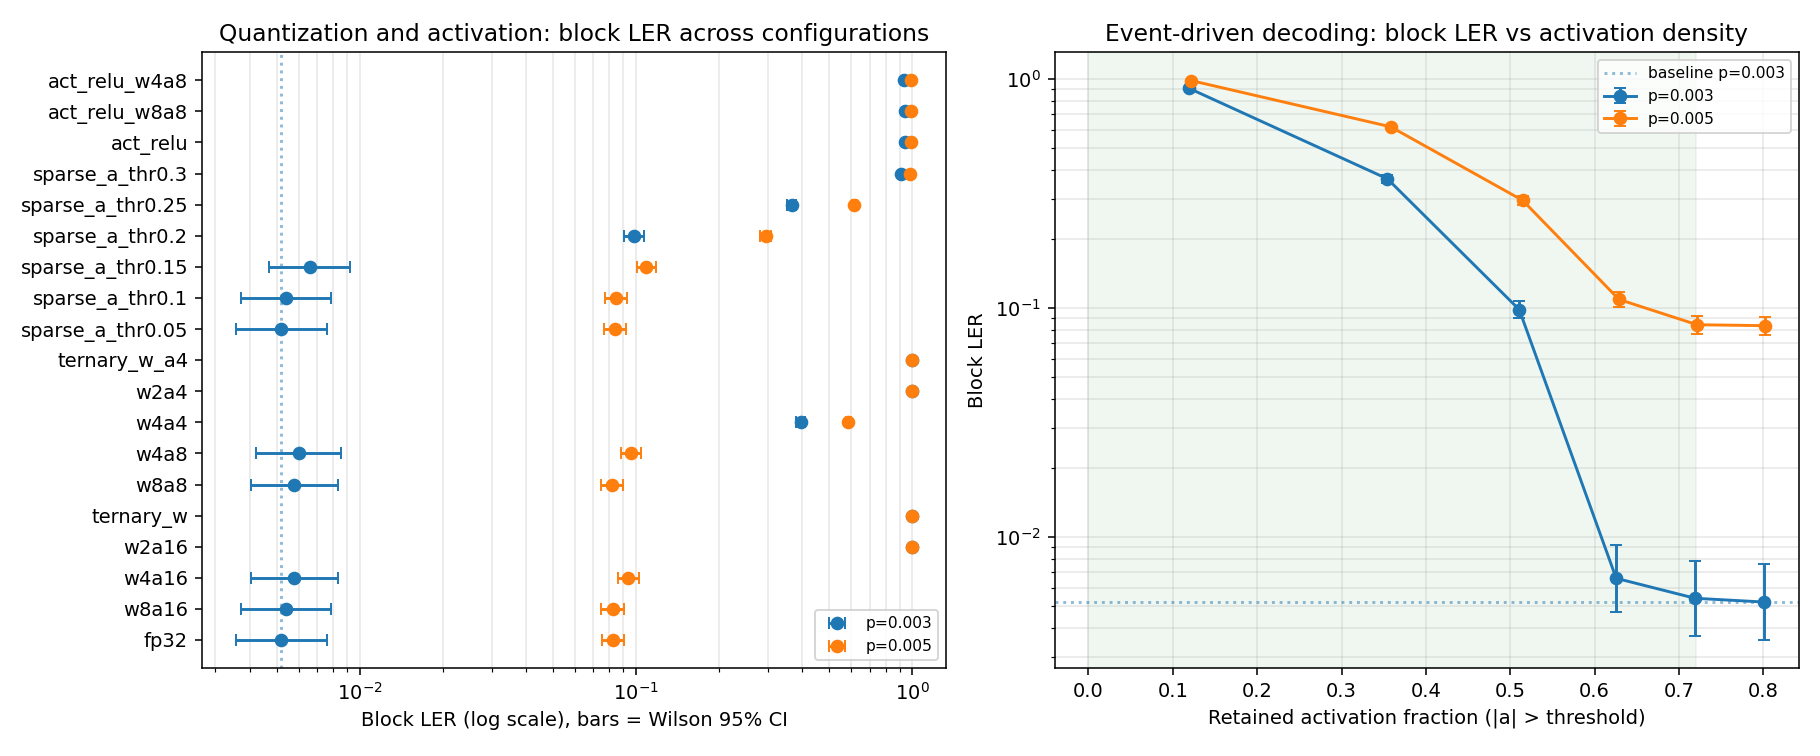
\includegraphics[width=0.50\textwidth]{figs/ntu_neuro_summary.png}
\caption{Post-training quantization and sparsity of the pretrained BB
transformer decoder. Left: block LER versus configuration (lower is
better) with the full-precision baseline marked. Right: accuracy as a
function of the retained activation fraction for the threshold-gating
scheme; the dashed line marks the full-precision LER. Error bars are Wilson
$95\%$ confidence intervals (5000 shots).}
\label{fig:neuro}
\end{figure*}
\subsection{Activation Sparsity}
To locate the accuracy cliff we sweep the magnitude threshold
$\tau\in\{0.05,0.10,0.15,0.20,0.25,0.30\}$ at $p{=}0.003$ and record the
retained activation fraction and the block LER (Table~\ref{tab:sparse} and
the right panel of Fig.~\ref{fig:neuro}). At $\tau{=}0.05$ and
$\tau{=}0.10$ about $20\%$ and $28\%$ of activations become exactly zero
with no measurable loss: the LER ($5.2$ and $5.4\times10^{-3}$) is
statistically indistinguishable from the FP32 baseline ($p{\approx}1.0$ and
$p{\approx}0.89$). At $\tau{=}0.15$ the density falls to $0.63$ at a LER of
$6.6\times10^{-3}$ ($p{\approx}0.36$), still consistent with the baseline.
The transition is then abrupt rather than gradual: at $\tau{=}0.20$ the LER
jumps to $9.8\times10^{-2}$ ($p{<}10^{-90}$) although the activation
fraction is still $0.51$, and beyond it the decoder keeps degrading
($3.7\times10^{-1}$ at $\tau{=}0.25$, $9.1\times10^{-1}$ at
$\tau{=}0.30$). The accuracy-preserving operating region therefore extends
to an activation fraction of about $0.6$--$0.7$ ($28$--$37\%$ of
activations gated off); pushing past it crosses a cliff, which is the
opposite of the graceful degradation a sparsity-aware accelerator would
require.
\begin{table}[t]
\caption{Activation-sparsity sweep at $p{=}0.003$ (5000 shots). $\tau$ is
the magnitude threshold, ``act.\ frac.'' the retained non-zero fraction,
and the final column the Wilson $95\%$ CI of the LER.}
\label{tab:sparse}
\centering
\footnotesize
\resizebox{\columnwidth}{!}{%
\begin{tabular}{ccccc}
\toprule
$\tau$ & Act.\ frac. & Gated off & LER at $p{=}0.003$ & $95\%$ CI \\
\midrule
0.05 & 0.80 & 20\% & $5.2\!\times\!10^{-3}$ & $[3.6,7.6]\!\times\!10^{-3}$ \\
0.10 & 0.72 & 28\% & $5.4\!\times\!10^{-3}$ & $[3.7,7.8]\!\times\!10^{-3}$ \\
0.15 & 0.63 & 37\% & $6.6\!\times\!10^{-3}$ & $[4.7,9.3]\!\times\!10^{-3}$ \\
0.20 & 0.51 & 49\% & $9.8\!\times\!10^{-2}$ & $[9.0,10.7]\!\times\!10^{-2}$ \\
0.25 & 0.35 & 65\% & $3.7\!\times\!10^{-1}$ & $[3.52,3.79]\!\times\!10^{-1}$ \\
0.30 & 0.12 & 88\% & $9.1\!\times\!10^{-1}$ & $[9.00,9.16]\!\times\!10^{-1}$ \\
\bottomrule
\end{tabular}}
\end{table}
\subsection{Activation-Function Replacement (Negative Result)}
Replacing every GELU/SiLU by a rectifier at inference time raises the LER
to $9.30\times10^{-1}$ at $p{=}0.003$, and combining the replacement with
W8A8 or W4A8 does not recover it ($9.28\times10^{-1}$ and
$9.25\times10^{-1}$). The pretrained model therefore depends strongly on
the smooth, gated activation behavior, and a purely post-training
substitution---the cheapest route to spiking hardware---is not viable.
This is consistent with recent findings that low-bit activations in QEC
decoders require quantization-aware training \cite{rethink2026}.
\subsection{Quantization-Aware Recovery}
The activation-replacement failure above is a post-training result, not
necessarily an intrinsic one. We therefore add a short quantization-aware
training (QAT) pass: keeping the pre-trained weights, we insert the target
nonlinearity (rectifier or LIF) and, where applicable, the low-bit
quantizers into the forward pass and fine-tune for 300 steps with a
straight-through estimator using AdamW (weight decay $1\times10^{-2}$),
learning rate $1\times10^{-4}$, and batch size 16--64 (the largest that
fits in memory for each configuration)---a minimal recipe with no schedule
and no early stopping. The cosine-scheduled variant anneals the learning
rate from $1\times10^{-4}$ to $2\times10^{-6}$ over the same 300 steps
with a 20-step linear warm-up. Table~\ref{tab:qat} shows
that the collapsed configurations recover from a near-total LER to a few
percent ($9.5\!\times\!10^{-1}\!\rightarrow\!3.4\!\times\!10^{-2}$ for the
rectifier, $9.9\!\times\!10^{-1}\!\rightarrow\!3.9\!\times\!10^{-2}$ for
LIF), whereas the already-accurate smooth-activation controls degrade
slightly (GELU $4.3\!\times\!10^{-3}\!\rightarrow\!1.9\!\times\!10^{-2}$)
because a fixed step perturbs a model already at the operating point. The
post-training constraint for event-driven conversion is thus a training problem,
closable by a brief QAT pass; but QAT should be used to \emph{reach}
event-driven operation rather than to re-compress an accurate
high-precision model, and it benefits from a learning-rate schedule or
early stopping. The recovered rates remain $6$--$10\times$ above the FP32
baseline, so this is a proof of principle rather than a converged
event-driven decoder.
Adding a cosine learning-rate schedule to the same pass (Fig.~\ref{fig:qat2})
deepens the recovery and closes the two walls the post-training study
exposed.
First, four-bit activations, which collapse in the post-training study
($3.9\!\times\!10^{-1}$ for the GELU model in Table~\ref{tab:quant} and
$9.3\!\times\!10^{-1}$ for the ReLU model in Table~\ref{tab:qat}), recover
to $2.2\!\times\!10^{-2}$---on par with the W4A8 control---so 4-bit
activations cease to be a wall once trained in the loop. Second, aggressive threshold gating at $\tau{=}0.20$, which
post-training collapses to $9.8\!\times\!10^{-2}$ at $51\%$ retained
activations, recovers to $1.6\!\times\!10^{-2}$ while retaining only
$\sim\!15\%$ of the activations---well past the post-training sparse
cliff. Quantization- and sparsity-aware training is therefore the route to
an aggressively quantized, event-driven decoder.
\begin{table}[t]
\caption{Short QAT pass (300 steps, straight-through estimator, 3000 shots,
$p{=}0.003$) on the configuration variants. ``Baseline'' is the
post-training model before fine-tuning, re-evaluated on this 3000-shot
set (hence small differences from the 5000-shot entries of
Table~\ref{tab:quant}); the last column is the lowest LER over the pass,
with its step. Rows marked $^{\dagger}$ use a cosine learning-rate
schedule.}
\label{tab:qat}
\centering
\footnotesize
\begin{tabular}{lcc}
\toprule
Configuration & Baseline LER & Best LER (step) \\
\midrule
GELU (control)        & $4.3\!\times\!10^{-3}$ & $1.9\!\times\!10^{-2}$ (150) \\
GELU + W4A8 (control) & $7.3\!\times\!10^{-3}$ & $2.3\!\times\!10^{-2}$ (100) \\
ReLU                  & $9.46\!\times\!10^{-1}$ & $3.4\!\times\!10^{-2}$ (100) \\
ReLU + W4A8           & $9.30\!\times\!10^{-1}$ & $4.4\!\times\!10^{-2}$ (250) \\
LIF                   & $9.89\!\times\!10^{-1}$ & $3.9\!\times\!10^{-2}$ (150) \\
ReLU + W4A4$^{\dagger}$ & $9.34\!\times\!10^{-1}$ & $2.2\!\times\!10^{-2}$ (300) \\
ReLU + W4A8, $\tau{=}0.20^{\dagger}$ & $9.30\!\times\!10^{-1}$ & $1.6\!\times\!10^{-2}$ (250) \\
\bottomrule
\end{tabular}
\end{table}
\begin{figure}[t]
\centering
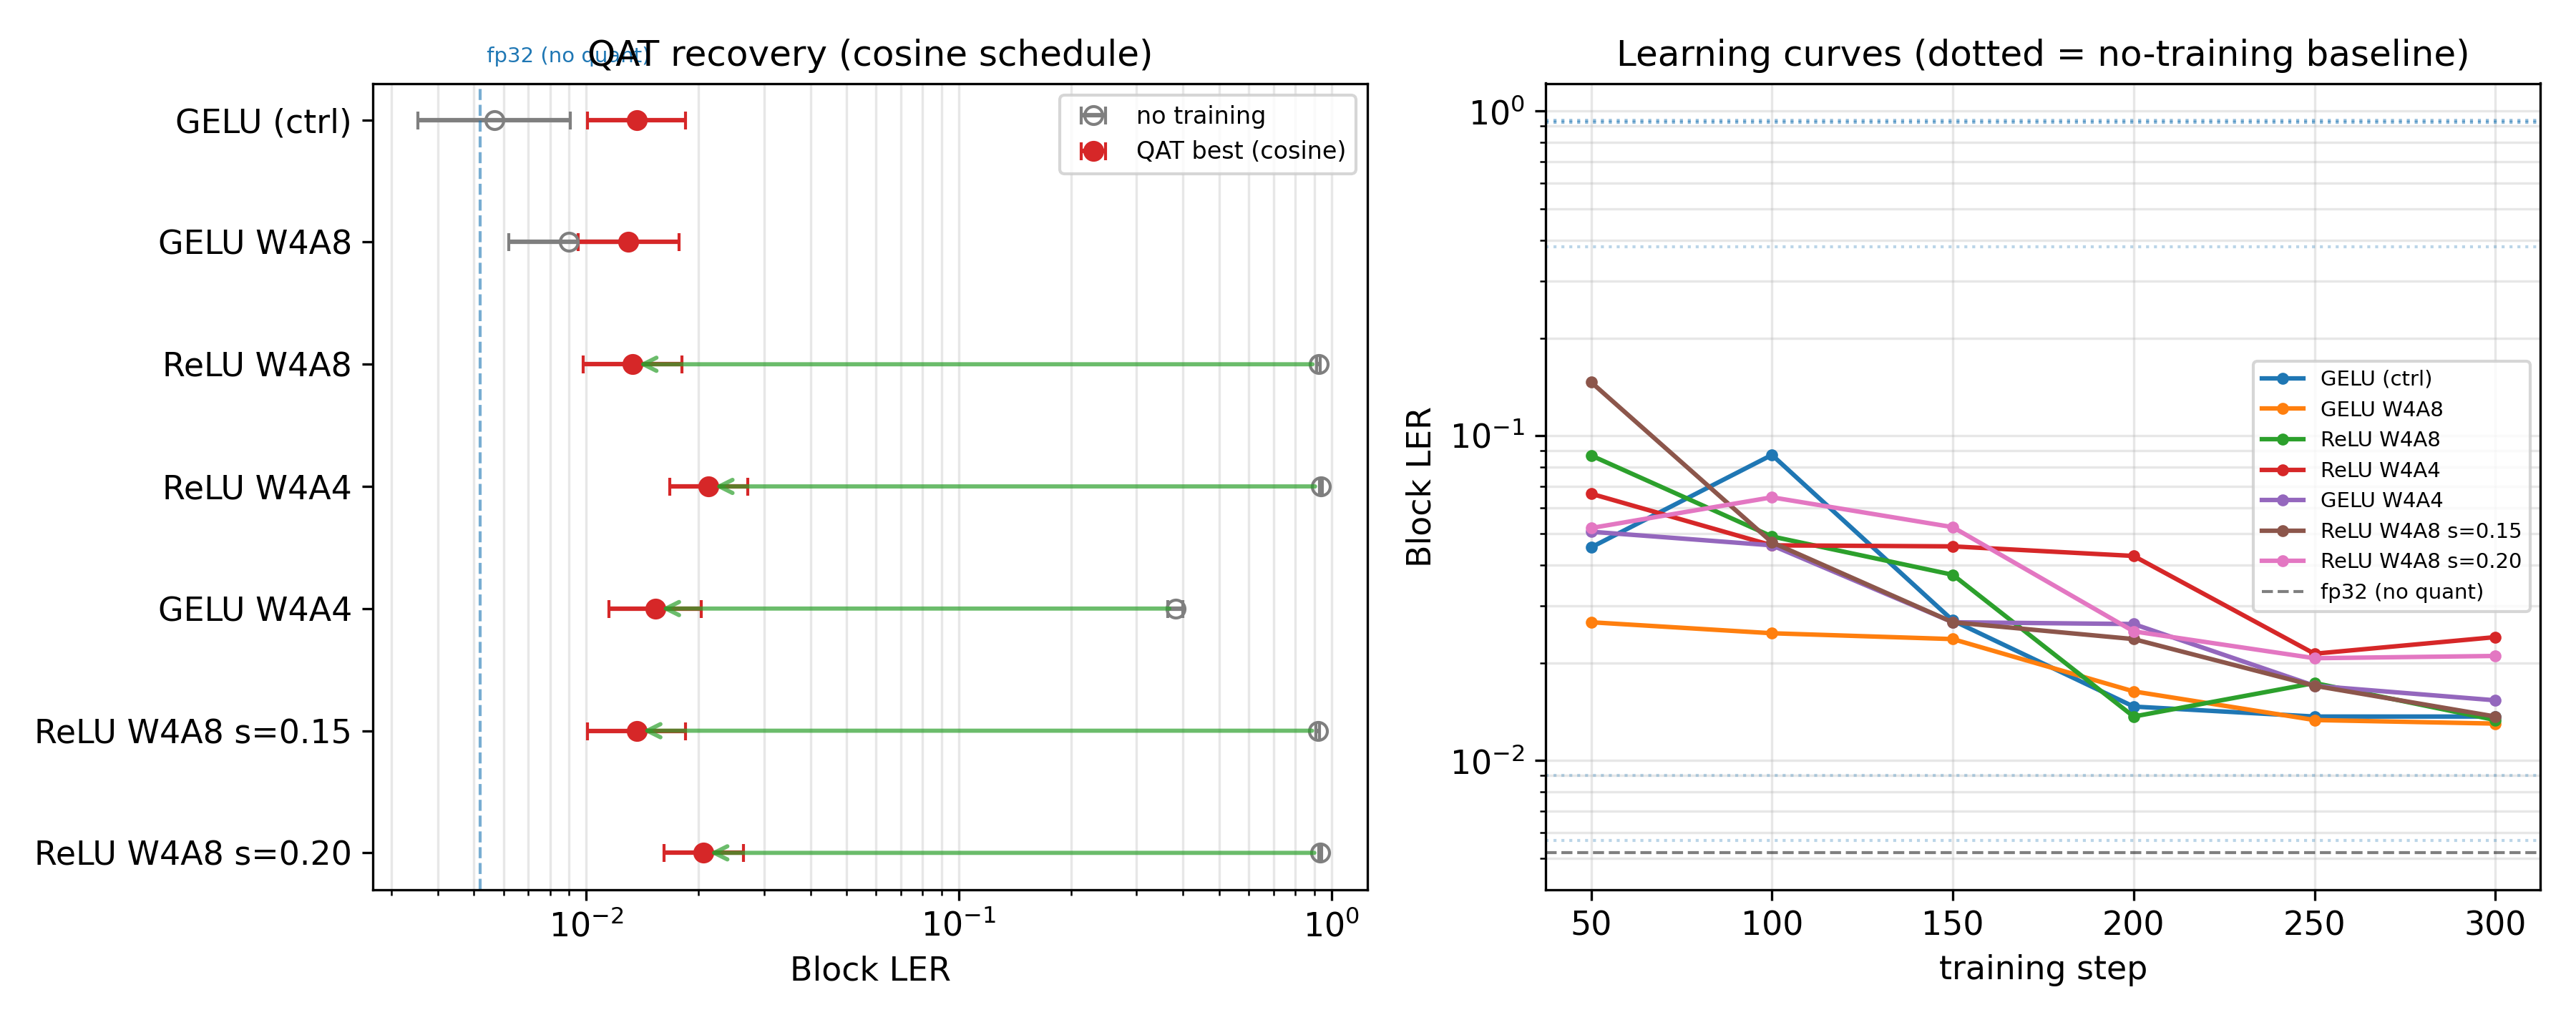
\includegraphics[width=0.66\linewidth]{figs/ntu_qat2_summary.png}
\caption{Quantization-aware recovery with a cosine learning-rate
schedule at $p{=}0.003$ (3000 shots). Left: post-training baseline
versus best LER over the pass, with Wilson $95\%$ confidence intervals.
Right: learning curves.}
\label{fig:qat2}
\end{figure}
\subsection{Hardware Cost Estimates}
Table~\ref{tab:hw} summarizes the estimated reductions. These figures are
analytical (we do not synthesize the model): weight memory follows from the
parameter count, and relative arithmetic energy from published
per-operation energies for 45\,nm CMOS at each bit width \cite{horowitz}.
Activation sparsity multiplies the operation count by $0.63$--$0.72$
(at $\tau{=}0.15$ and $0.10$).
The energy numbers are a first-order, node-agnostic proxy. At a modern
accelerator node (7--5\,nm) the arithmetic per-operation energy falls by a
factor of a few relative to 45\,nm \cite{sze2017,agrawal2021}, while
off-chip data movement remains one to two orders of magnitude above
arithmetic \cite{horowitz,sze2017}; the \emph{relative} savings we report
are governed to leading order by operand width and data movement, which is
qualitatively process-independent. We therefore use the classical figures
only to rank the configurations (FP32 $\gg$ W8A8 $>$ W4A8) and do not
claim node-accurate absolute energies; a target-node or cryogenic energy
model would change the absolute scale but not the ordering.
The projected footprint can be bounded from the
parameter count. At W4A8 the weights occupy 18\,MB, which
exceeds the block-RAM capacity of a mid-range FPGA (a few MB), so they must
be streamed from off-chip memory or held in an HBM-equipped device: the
decoder is \emph{memory-bound}, sized by the bandwidth needed to feed its
MAC lanes rather than by compute. Low-bit weights therefore help directly
(cutting the streamed weight volume by $4$--$8\times$), whereas activation
sparsity helps only in proportion to the accelerator's ability to skip the
corresponding MACs and activation fetches. A pipelined array of $L$ MAC
lanes at frequency $f$ sustains at most $Lf$ MAC/s, so the per-syndrome
latency scales as the MACs per forward pass divided by $Lf$; a real-time
budget therefore needs a wide array \emph{combined} with the compression
above. A synthesis-level study is left to future work.
\begin{table}[t]
\caption{Analytical hardware cost estimates relative to the FP32
reference. Weight memory follows from the 35.98M-parameter count; relative
arithmetic energy uses published per-MAC energies \cite{horowitz};
sparsity multiplies the operation count by $0.63$--$0.72$. Estimates only,
not measured device figures.}
\label{tab:hw}
\centering
\footnotesize
\resizebox{\columnwidth}{!}{%
\begin{tabular}{lcccc}
\toprule
Configuration & Weight & Weight mem. & Rel. MAC & Rel. ops \\
              & bits   & (MB)        & energy   & (sparsity) \\
\midrule
FP32 (reference) & 32 & 143.9 & 1.0   & 1.0 \\
W8A8             & 8  & 36.0  & 0.058 & 1.0 \\
W4A8             & 4  & 18.0  & 0.033 & 1.0 \\
W4A8 + sparsity  & 4  & 18.0  & 0.033 & 0.63--0.72 \\
\bottomrule
\end{tabular}}
\end{table}
\section{Discussion}\label{sec:disc}
Our results delineate the boundary between what post-training compression
can and cannot achieve for BB neural decoding.

\textbf{Practical operating point.} A decoder at W4A8 with a threshold rule
that zeroes about $28$--$37\%$ of activations retains the accuracy of the
floating-point model within sampling uncertainty while reducing arithmetic
width by more than $2\times$ and weight memory by $8\times$ (Table~\ref{tab:hw}).
This is a realistic target for integer or event-driven accelerators, and it
requires no retraining, which matters given the cost of training QEC
decoders.

\textbf{Activation precision dominates.} The asymmetry between weight and
activation sensitivity (Table~\ref{tab:quant}) is the most actionable
observation: effort should be spent on activation representation, not on
weight compression. Weight quantization can be pushed to 4 bits, but 4-bit
activations are not viable without retraining.

\textbf{Positioning.} Recent work on surface-code decoders reaches INT4
operating points through a compression pipeline that combines pruning and
quantization-aware training, and reports that INT4 is a prerequisite for
micron-scale latency on FPGA \cite{rethink2026}. Our study is complementary
and, to our knowledge, is the first to characterize the \emph{post-training}
boundary for a QLDPC (bivariate bicycle) decoder: we quantify how far
conventional compression proceeds without retraining, locate the
activation-precision and activation-density cliffs, and show where that
route stops. This complements, rather than duplicates, QAT-based pipelines
by providing the accuracy-vs-cost reference against which they should be
compared for QLDPC codes. Table~\ref{tab:prior} summarizes the relation to
the closest prior work.
\begin{table}[t]
\caption{Relation to prior work on compressing neural QEC decoders. ``+ QAT'' denotes the 300-step quantization-aware-training probe of Table~\ref{tab:qat}.}
\label{tab:prior}
\centering
\footnotesize
\setlength{\tabcolsep}{2.5pt}
\begin{tabular}{llcc}
\toprule
Work & Code / decoder & Compression & Retrain \\
\midrule
Blue \emph{et al.}\ \cite{blue2026} & BB72 transformer & FP32 & --- \\
Yan \emph{et al.}\ \cite{rethink2026} & surface code NN & INT4 (QAT) & yes \\
\textbf{This work} & BB72 transformer & W4A8{,} $28$--$37\%$ sparse & no (+ QAT) \\
\bottomrule
\end{tabular}
\end{table}
\textbf{Towards event-driven decoders.} The activation-replacement result
shows that a truly event-driven or spiking decoder is not obtainable by
post-hoc conversion, but the QAT recovery result (Table~\ref{tab:qat})
shows the gap is closable: a brief fine-tuning pass with the target
nonlinearity in the loop moves the collapsed variants from near-total
failure to a few percent LER. Because spiking hardware reaches its
low-power regime only with rectifier-like, sparse activations, the route
to a deployable event-driven decoder is quantization- and sparsity-aware
training with the target nonlinearity and sparsity pattern in the loop,
followed by the low-bit, sparse operating point characterized here.

\textbf{Limitations.} We evaluate a single pretrained checkpoint and one
code instance, use a 5000-shot budget per noise level (3000 for the
quantization-aware training study), and simulate
integer arithmetic without modeling accumulator bit-widths or the exact
rounding of a target datapath. The confidence intervals at low $p$ are
wide, so small differences between the high-precision configurations cannot
be resolved at this sample size. The hardware figures are analytical and do
not include latency, area, or synthesis results; the sparsity figure is an
upper bound on skippable MACs, and realized speedups depend on the
accelerator's ability to exploit unstructured sparsity.
\section{Conclusion}
We characterized hardware-oriented compression of a transformer decoder
for BB codes. Post-training, W8A8 preserves accuracy within sampling
uncertainty and W4A8 degrades it only marginally, while activation
precision dominates and a magnitude threshold removes $28$--$37\%$ of
activations without measurable loss. A naive rectifier replacement
severely degrades decoding, so weight-only post-training quantization is
insufficient for event-driven operation; a short QAT pass nevertheless
recovers the collapsed configurations by more than an order of magnitude,
showing the target nonlinearity should be trained rather than converted
post-hoc. These results give a practical compression recipe and accuracy
reference for low-power BB neural decoders, motivating our ongoing work on
trained event-driven decoding.
\section*{Acknowledgment}
The author thanks the developers of the open-source pretrained BB
transformer decoder, whose released model and code made this study
possible; compute was provided by the Kaggle notebook platform.
\begin{thebibliography}{00}\footnotesize\setlength{\itemsep}{0pt}\setlength{\parsep}{0pt}\setlength{\parskip}{0pt}
\bibitem{dennis2002} E. Dennis \emph{et al.},
``Topological quantum memory,'' \emph{J. Math. Phys.}, vol. 43, no. 9,
pp. 4452--4505, 2002.
\bibitem{google2023} Google Quantum AI, ``Suppressing quantum errors by
scaling a surface code logical qubit,'' \emph{Nature}, vol. 614,
pp. 676--681, 2023.
\bibitem{bravyi2024} S. Bravyi \emph{et al.}, ``High-threshold and
low-overhead fault-tolerant quantum memory,'' \emph{Nature}, vol. 627,
pp. 778--782, 2024.
\bibitem{blue2026} J. Blue \emph{et al.},
``Machine learning decoding of circuit-level noise for bivariate bicycle
codes,'' \emph{Quantum}, vol. 10, p. 2149, 2026.
\bibitem{rethink2026} G. Yan, S. Li, and Y. Du, ``Rethink the role of
neural decoders in quantum error correction,'' arXiv:2605.12046, 2026.
\bibitem{horowitz} M. Horowitz, ``Computing's energy problem (and what we
can do about it),'' in \emph{IEEE Int. Solid-State Circuits Conf. (ISSCC)},
2014, pp. 10--14.
\bibitem{sze2017} V. Sze \emph{et al.},
``Efficient processing of deep neural networks: A tutorial and survey,''
\emph{Proc. IEEE}, vol. 105, no. 12, pp. 2295--2329, 2017.
\bibitem{agrawal2021} A. Agrawal \emph{et al.}, ``9.1 A 7nm 4-core AI chip
with 25.6TFLOPS hybrid FP8 training, 102.4TOPS INT4 inference and
workload-aware throttling,'' in \emph{IEEE Int. Solid-State Circuits Conf.
(ISSCC)}, 2021, vol. 64, pp. 144--146.
\bibitem{stimb} C. Gidney, ``Stim: A fast stabilizer circuit simulator,''
\emph{Quantum}, vol. 5, p. 497, 2021.
\bibitem{LiuDiff25}
Z. Liu, A. Gong, and B. K. Clark, ``Decoding quantum low density parity check codes with diffusion,'' arXiv:2509.22347, Sep. 2025.
\bibitem{CaoGen25}
H. Cao \emph{et al.}, ``Generative decoding for quantum error-correcting codes,'' arXiv:2503.21374, Mar. 2025.
\bibitem{DasHPCA22}
P. Das \emph{et al.}, ``Accurate, fast, and scalable error-decoding for fault-tolerant quantum computers,'' in \emph{Proc. HPCA}, 2022, pp. 259--273.
\bibitem{MiMueller25}
X. Mi and F. Mueller, ``Toward uncertainty-aware and generalizable neural decoding for quantum LDPC codes,'' arXiv:2510.06257, 2025
\end{thebibliography}
\end{document}
